在不同的内核形式之间进行选择,很大程度上取决于个人偏好,并且很大程度上受到以前使用其他并行编程模型和语言的经验的影响。\par

选择特定内核形式的另一个主要原因是,公开内核所需的功能的唯一形式。不幸的是,在开发开始之前很难确定需要哪些功能——特别是当我们不熟悉不同的内核形式,以及它们与各种类是如何交互时。\par

为了帮助读者们进行选择,我们根据自己的经验构建了两个指南。可以参考这些经验法则,但最好的方法是选择不同的内核形式进行编写,对不同的方式进行测试和了解,从而在开发应用程序时选择最合适的内核形式和开发方式。\par

第一个指南是如图4-26所示的流程图,选择基于的内核形式\par

\begin{itemize}
	\item 是否有并行编程的经验
	\item 是从头编写新代码,还是移植用现有的并行程序
	\item 是包含嵌套的并行,还是在内核函数的不同实例之间重用数据
	\item 是用SYCL编写新内核是为了最大化性能,还是为了提高代码的可移植性,使用一种比底层的语言更高效的表示并行性
\end{itemize}

\hspace*{\fill} \par %插入空行
图4-26 帮助我们为内核选择正确的形式
\begin{center}
	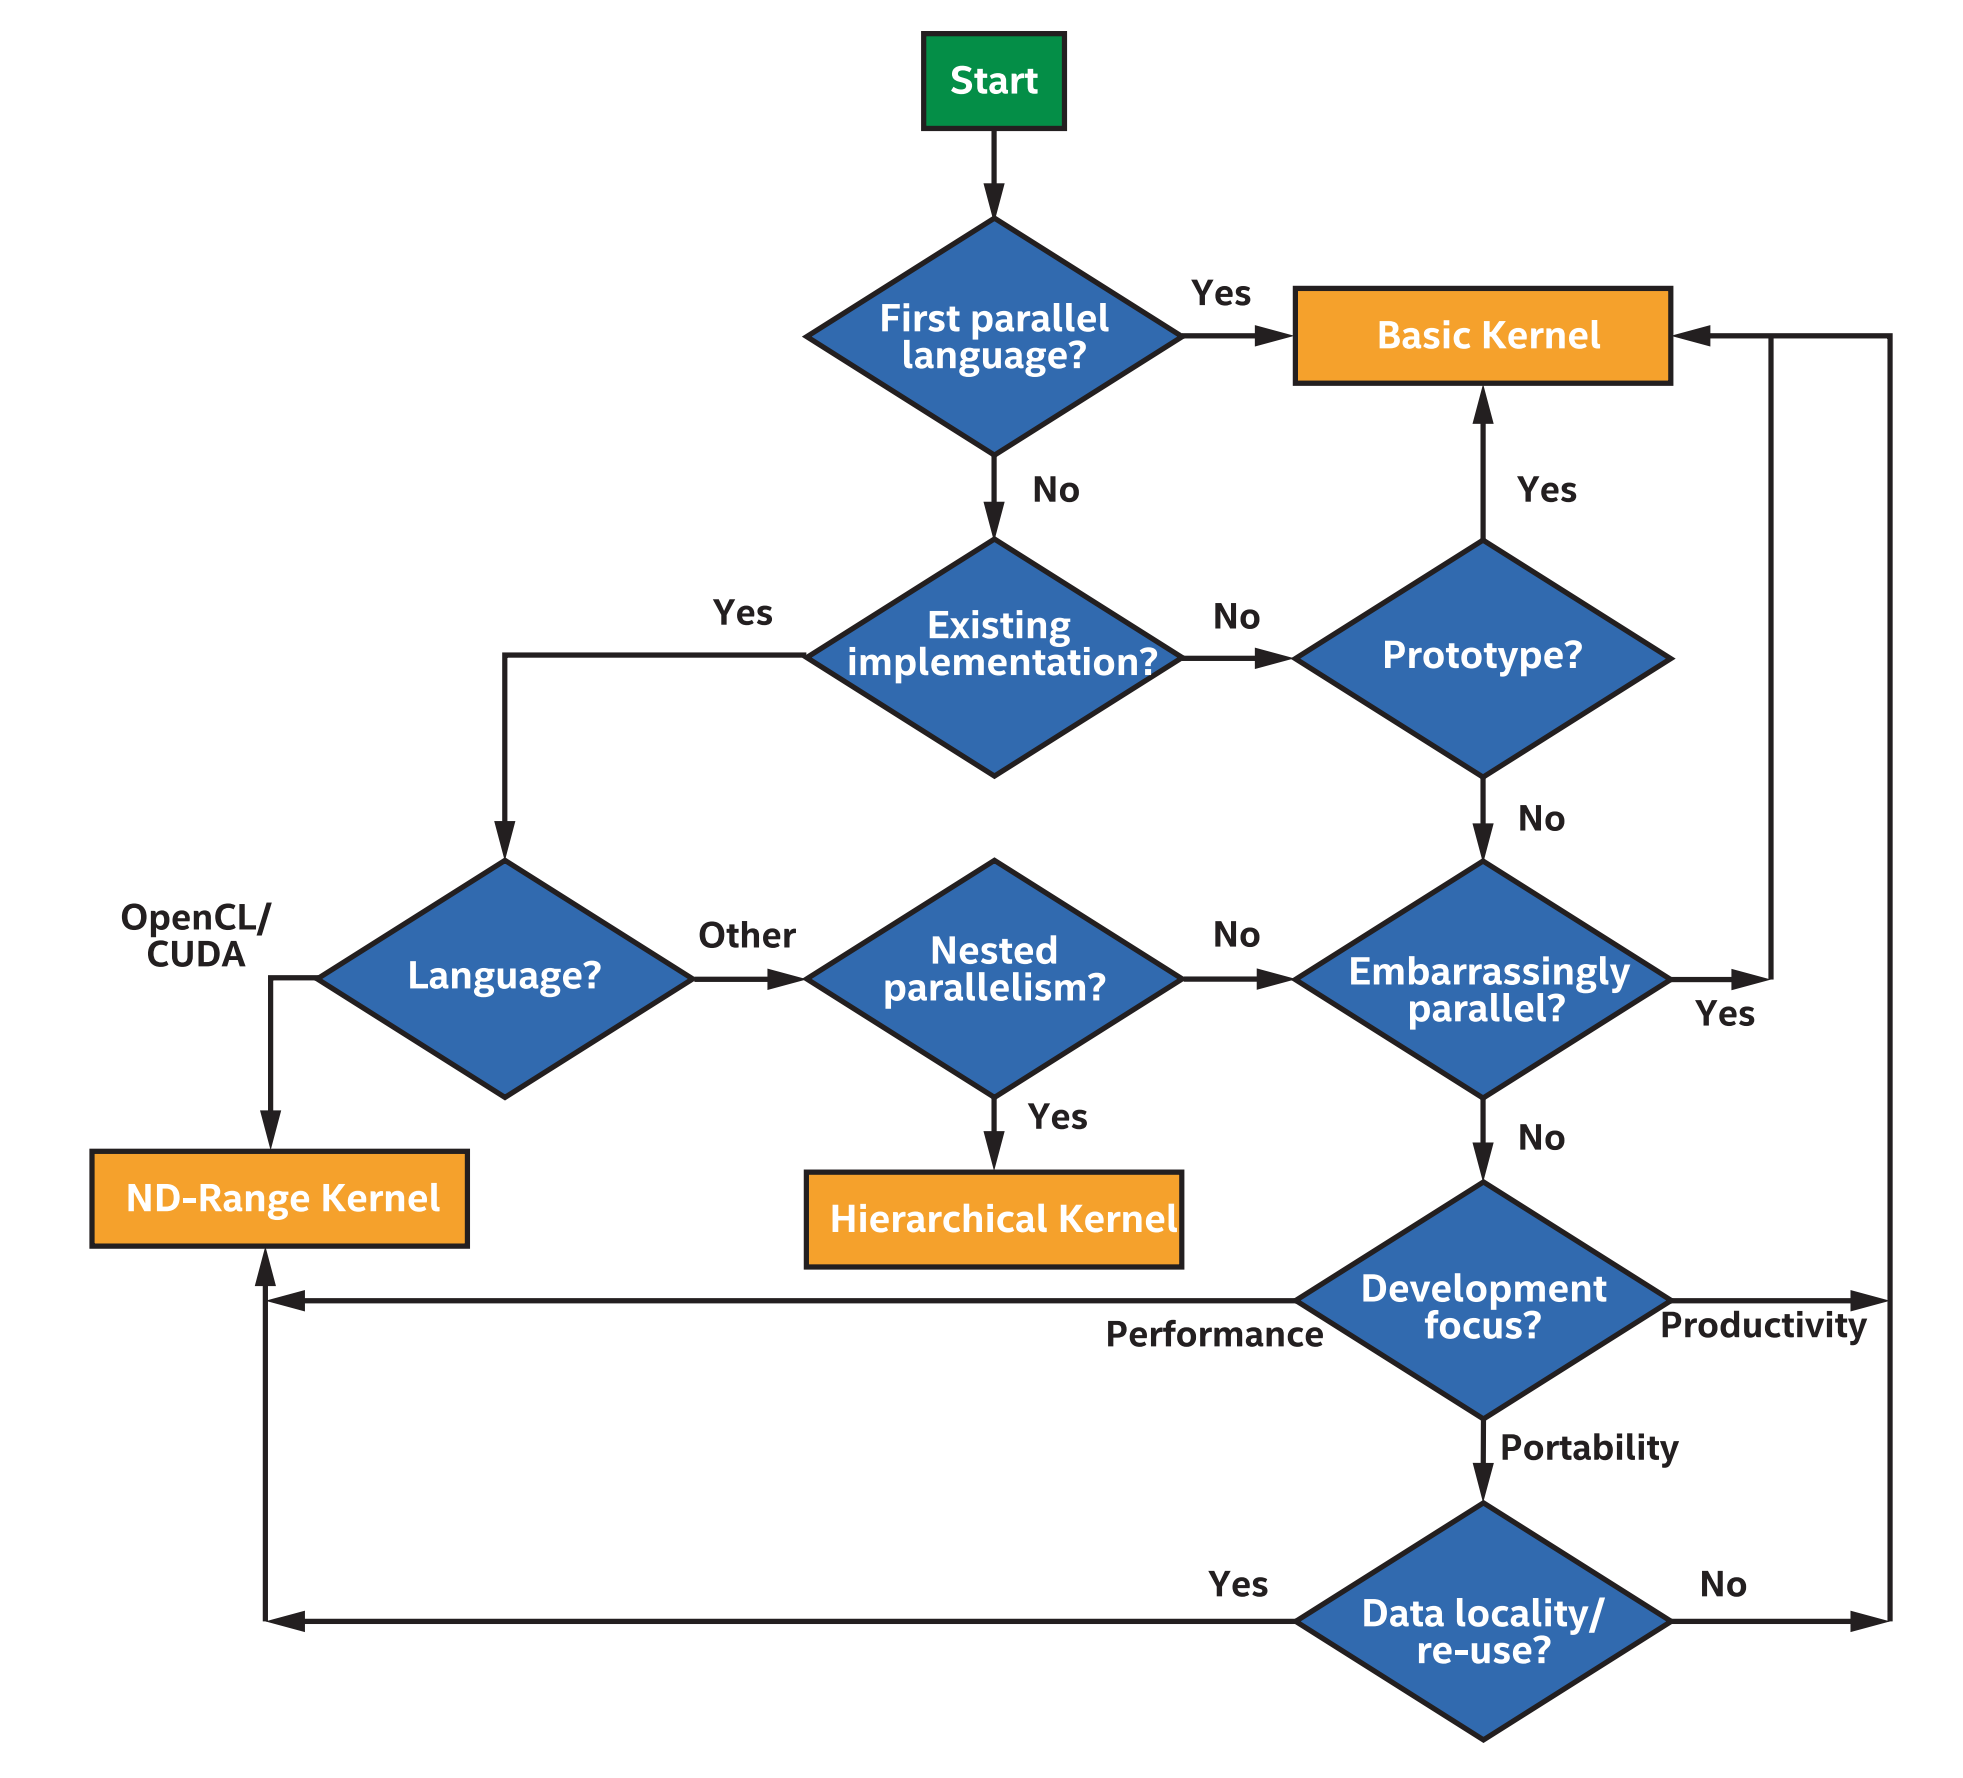
\includegraphics[width=0.8\textwidth]{content/chapter-4/images/7}
\end{center}

第二个指南是图4-27中的表格,它总结了每种内核形式公开的功能。值得注意的是,这个表反映了DPC++在本书出版时的状态,随着语言的发展,每个内核形式可用的特性应该会发生变化。我们预计基本趋势将保持不变:基本的数据并行内核不会公开位置感知特性,显式的ND-Range内核会公开所有支持性能的特性,分层内核在公开特性方面会落后于显式的ND-Range内核,但是它们对这些特性的表达将使用更高层次的抽象。\par

\hspace*{\fill} \par %插入空行
图4-27 每种内核形式的特性
\begin{table}[H]
	\begin{tabular}{|l|c|c|c|}
		\hline
		\textbf{特性}                           & \multicolumn{1}{l|}{\textbf{基本内核}} & \multicolumn{1}{l|}{\textbf{ND-Range内核}} & \multicolumn{1}{l|}{\textbf{层次内核}} \\ \hline
		\textbf{工作组本地内存}           & No                                         & Yes                                           & Yes                                              \\ \hline
		\textbf{工作组栅栏}               & No                                         & Yes                                           & Yes                                              \\ \hline
		\textbf{子工作组}                        & No                                         & Yes                                           & No                                               \\ \hline
		\textbf{工作组函数(比如:scan,reduce)} & No                                         & Yes                                           & No                                               \\ \hline
	\end{tabular}
\end{table}




